\graphicspath{{content/11-reference/images/}}

\chapter{Référence}

\section{Utilisation de Rsnap}

%\subsection{Créer une mission}
\begin{figure}
  \begin{center}
    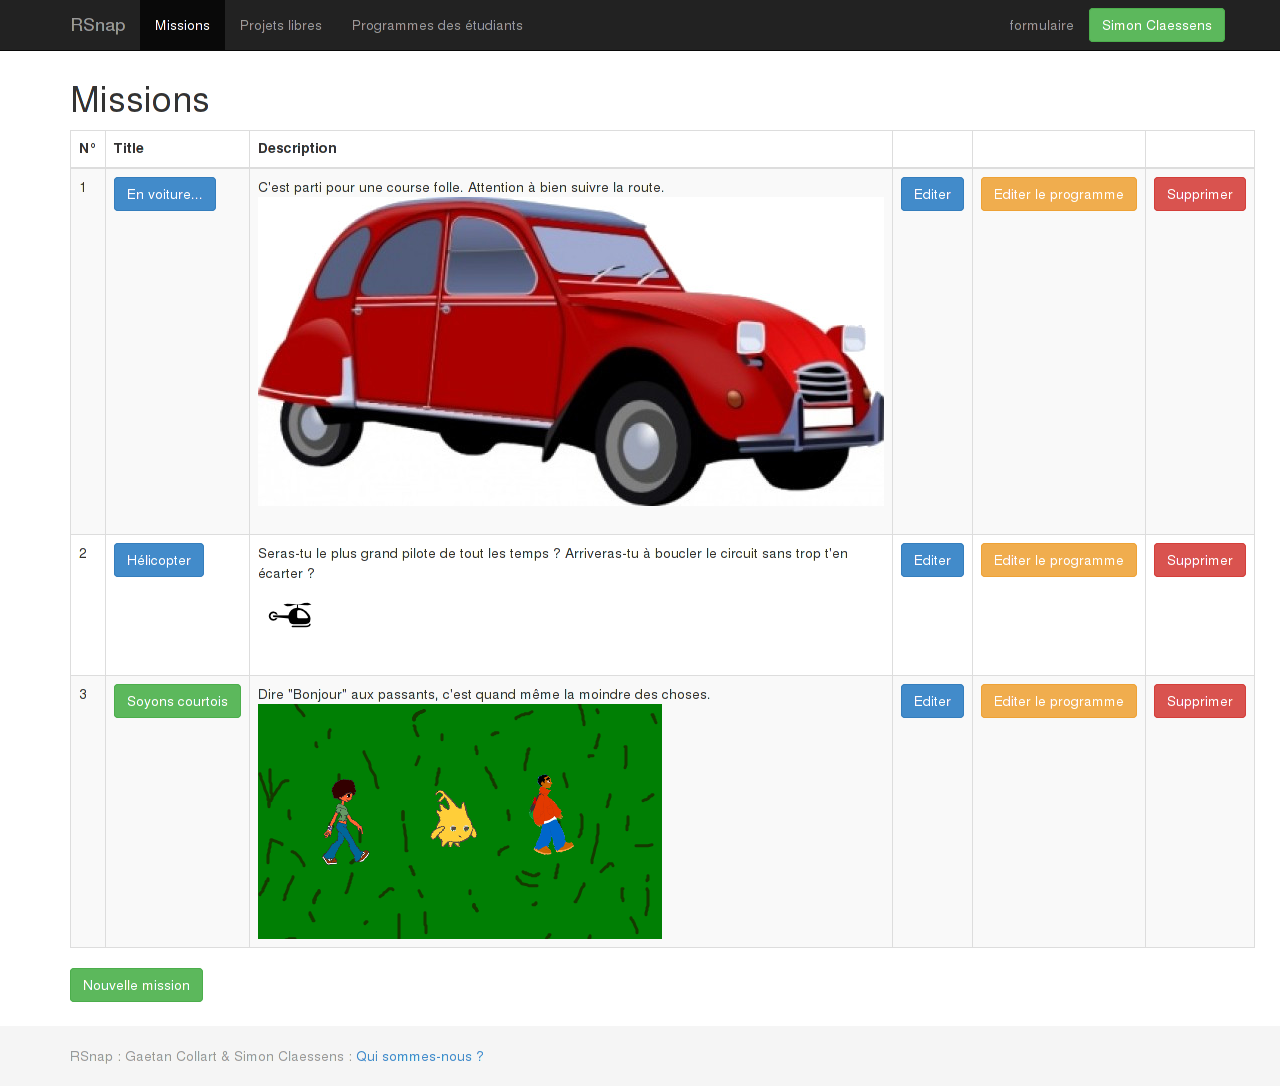
\includegraphics[width=\textwidth]{creer-mission-1}
    \caption{Page des missions}
    \label{fig:creer-mission-1}
  \end{center}
\end{figure}
\begin{figure}
  \begin{center}
    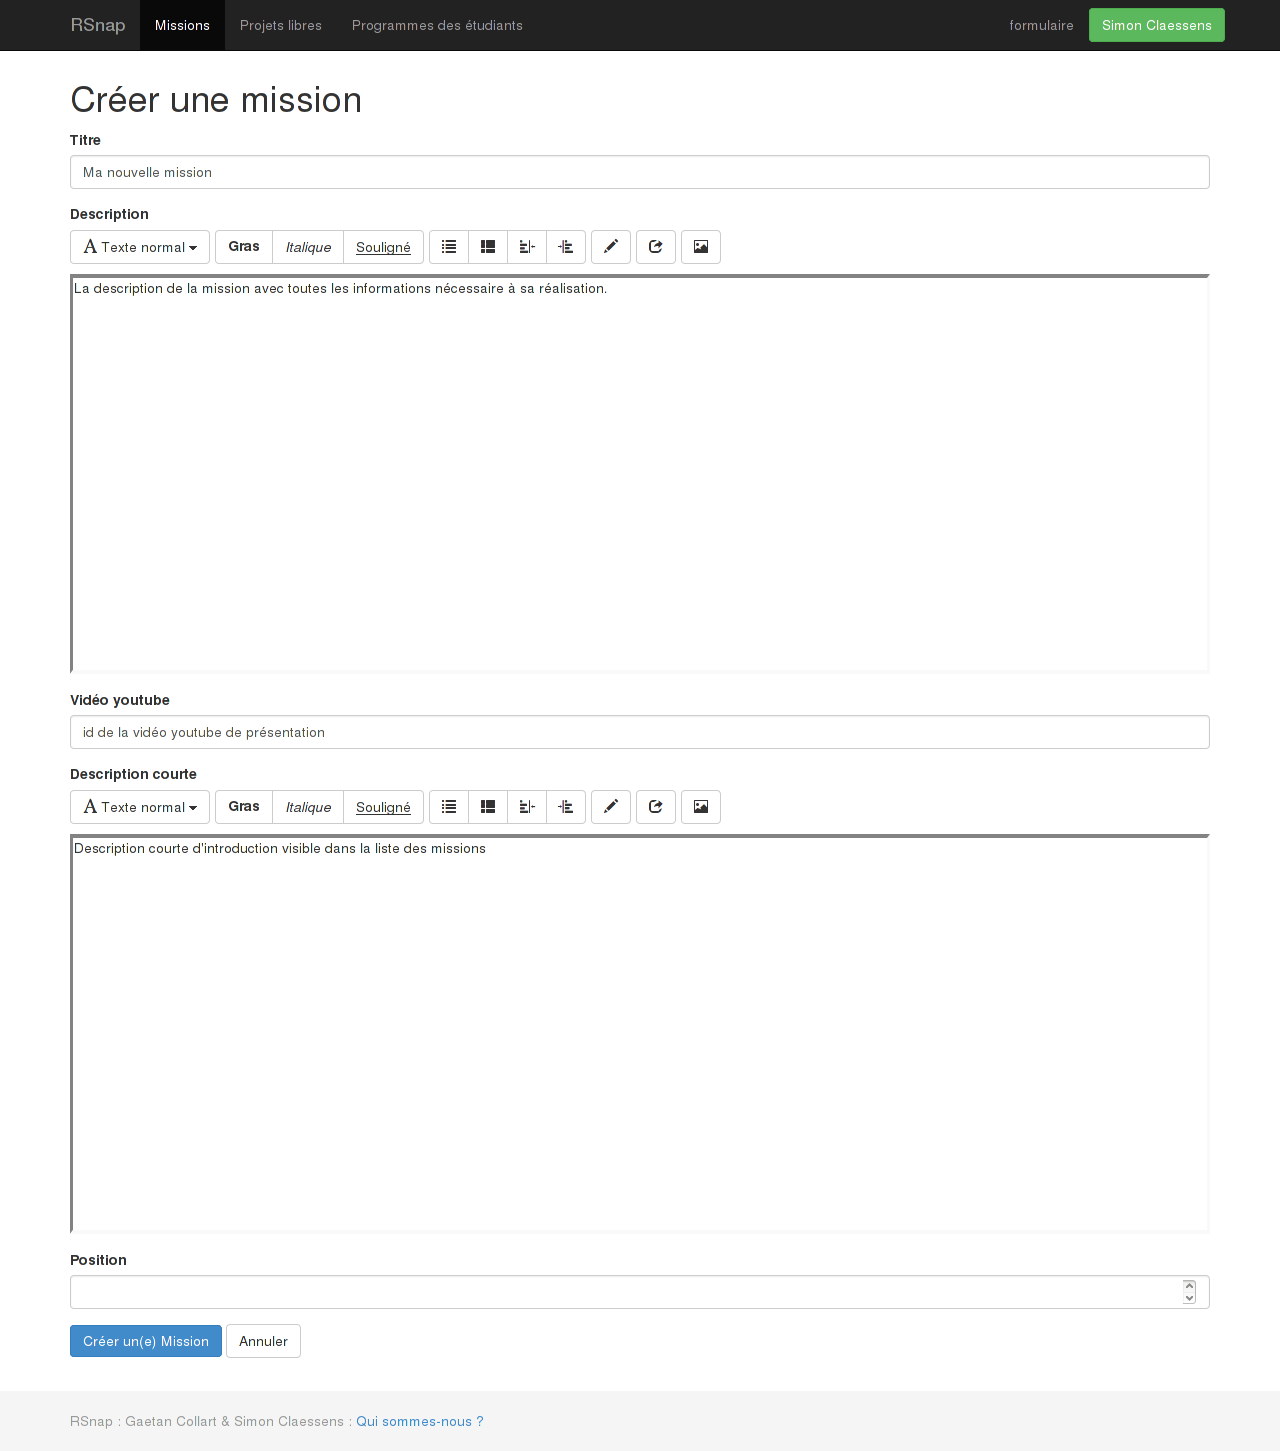
\includegraphics[width=\textwidth]{creer-mission-2}
    \caption{Création des informations de la mission}
    \label{fig:creer-mission-2}
  \end{center}
\end{figure}
\begin{figure}
  \begin{center}
    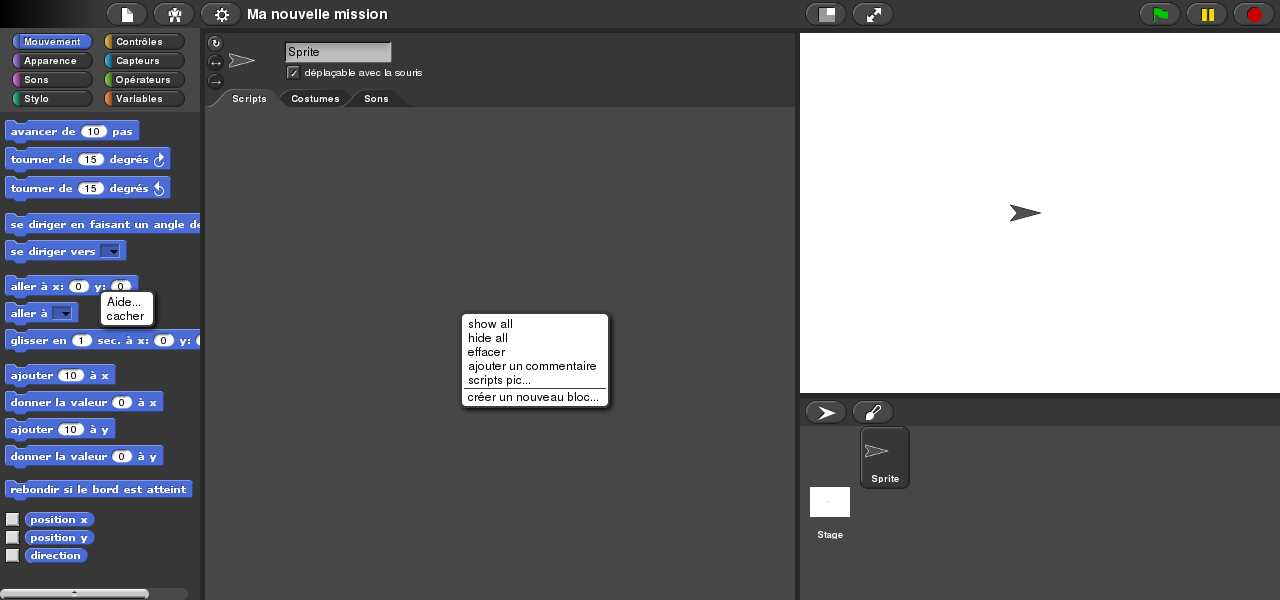
\includegraphics[width=\textwidth]{creer-mission-3}
    \caption{Création du programme de la mission}
    \label{fig:creer-mission-3}
  \end{center}
\end{figure}

%\subsection{Ordonner les missions}
\begin{figure}
  \begin{center}
    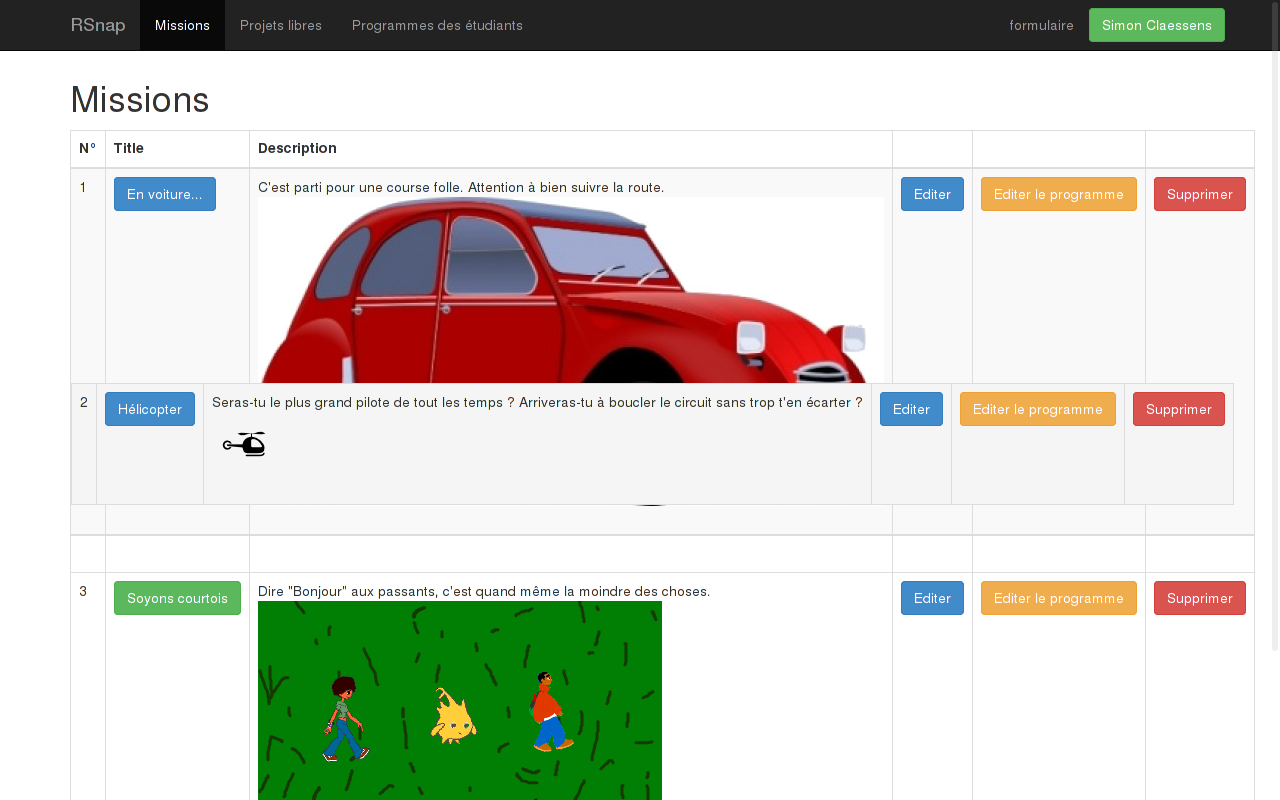
\includegraphics[width=\textwidth]{mission-order}
    \caption{Ordonner les missions}
    \label{fig:mission-order}
  \end{center}
\end{figure}

%\subsection{Corriger une mission}
\begin{figure}
  \begin{center}
    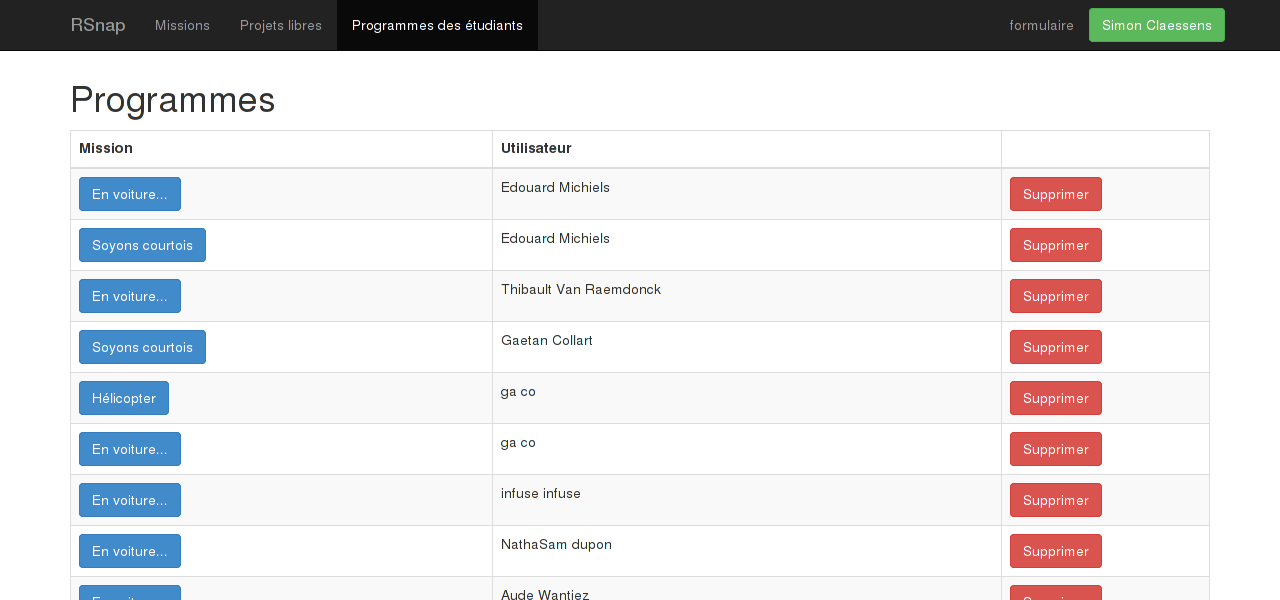
\includegraphics[width=\textwidth]{corriger-prog-1}
    \caption{Page des programmes des élèves}
    \label{fig:corriger-prog-1}
  \end{center}
\end{figure}
\begin{figure}
  \begin{center}
    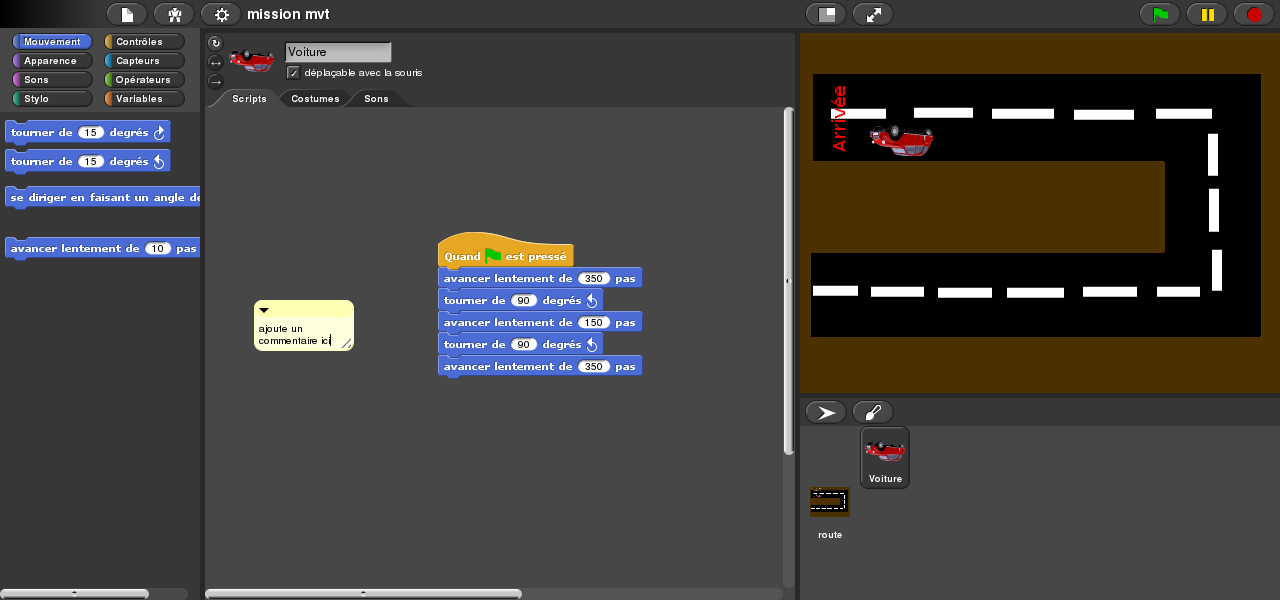
\includegraphics[width=\textwidth]{corriger-prog-2}
    \caption{Correction du programme}
    \label{fig:corriger-prog-2}
  \end{center}
\end{figure}

%\subsection{Réaliser une mission}
\begin{figure}
  \begin{center}
    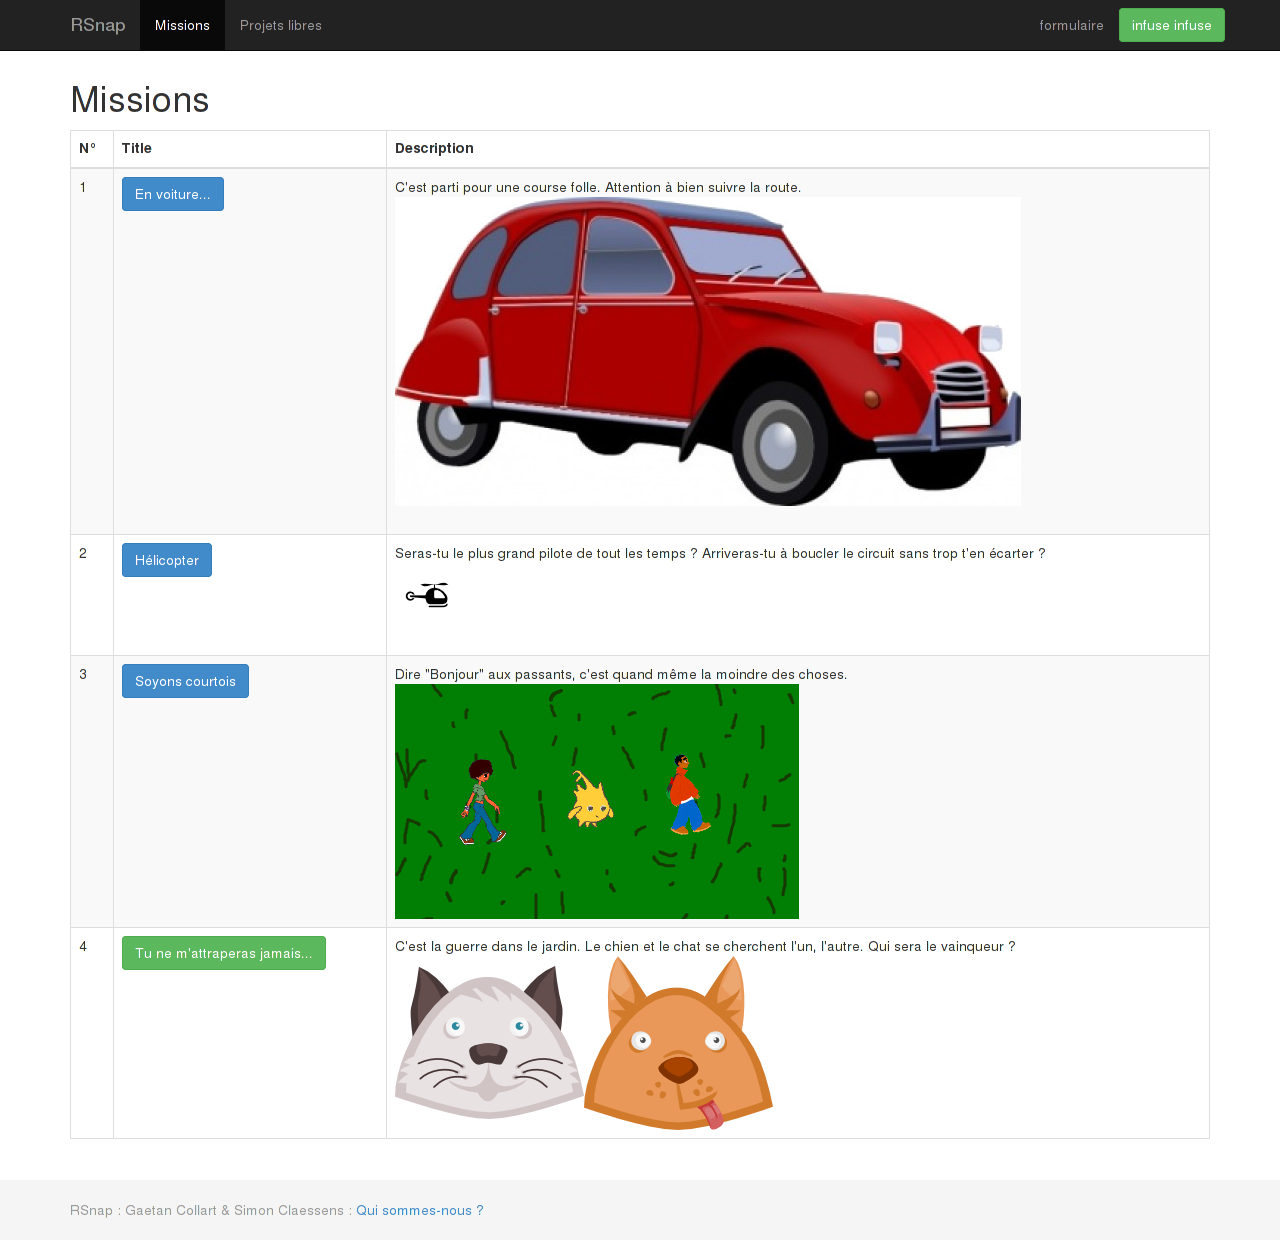
\includegraphics[width=\textwidth]{realiser-mission-1}
    \caption{Page des missions}
    \label{fig:realiser-mission-1}
  \end{center}
\end{figure}
\begin{figure}
  \begin{center}
    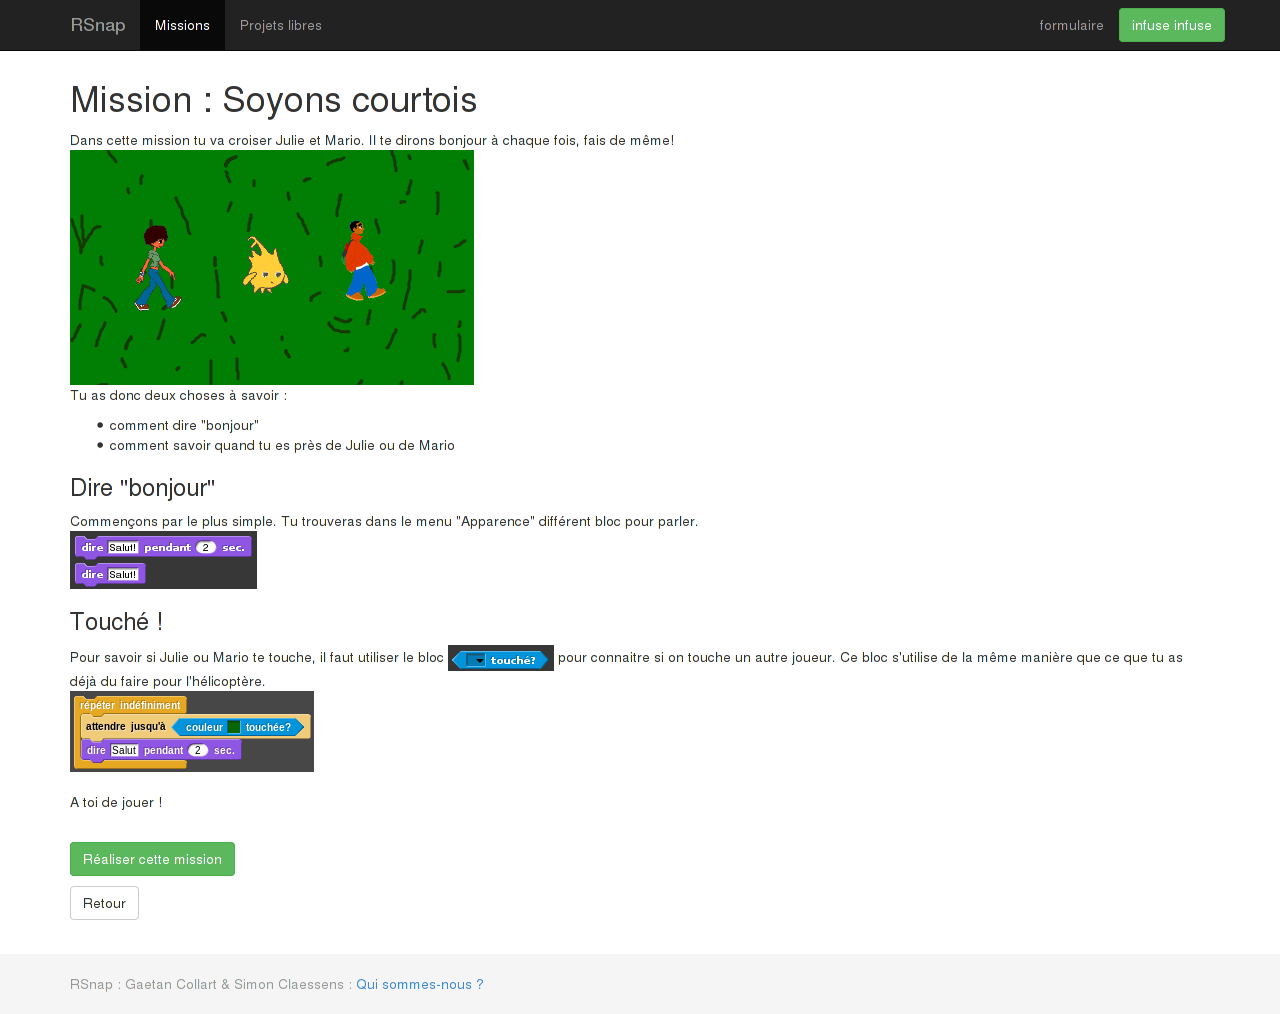
\includegraphics[width=\textwidth]{realiser-mission-2}
    \caption{Description de la mission}
    \label{fig:realiser-mission-2}
  \end{center}
\end{figure}
\begin{figure}
  \begin{center}
    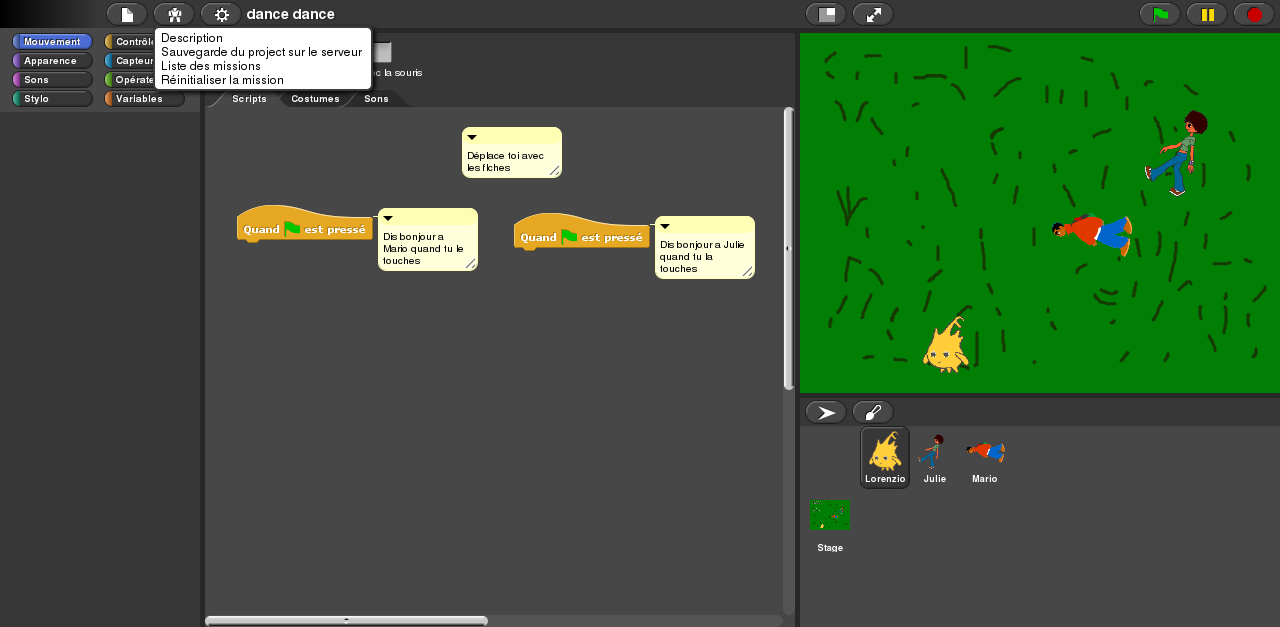
\includegraphics[width=\textwidth]{realiser-mission-3}
    \caption{Réalisation de la mission}
    \label{fig:realiser-mission-3}
  \end{center}
\end{figure}

%\subsection{Réaliser un projet libre}
\begin{figure}
  \begin{center}
    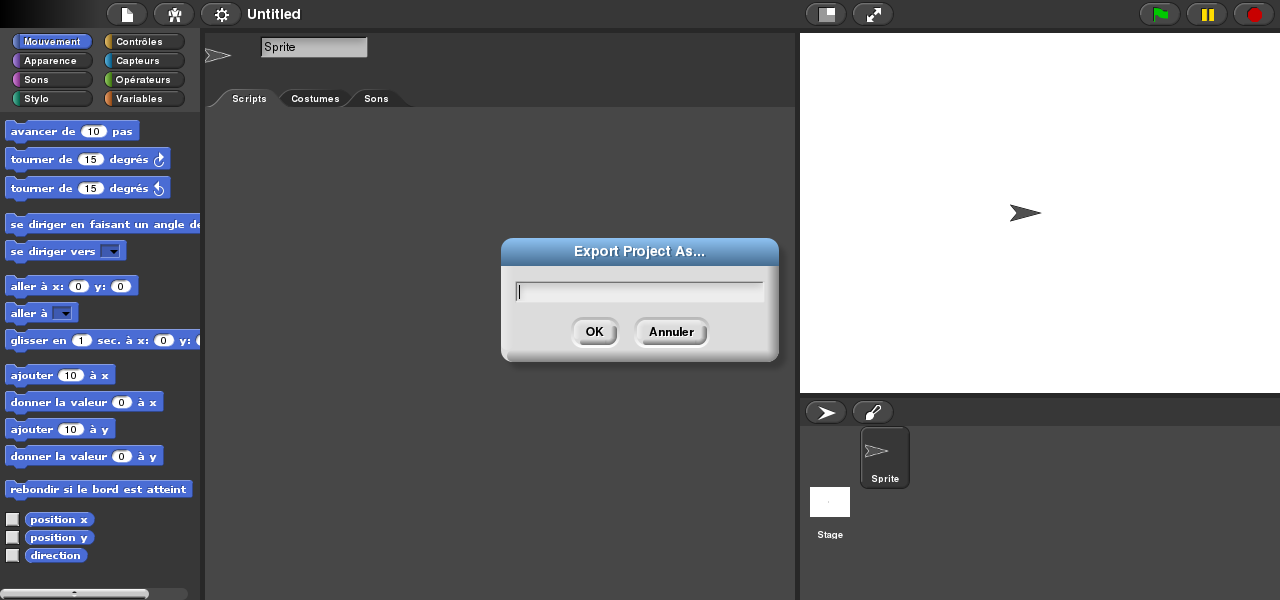
\includegraphics[width=\textwidth]{projet-1}
    \caption{Page des projets libres}
    \label{fig:projet-1}
  \end{center}
\end{figure}
\begin{figure}
  \begin{center}
    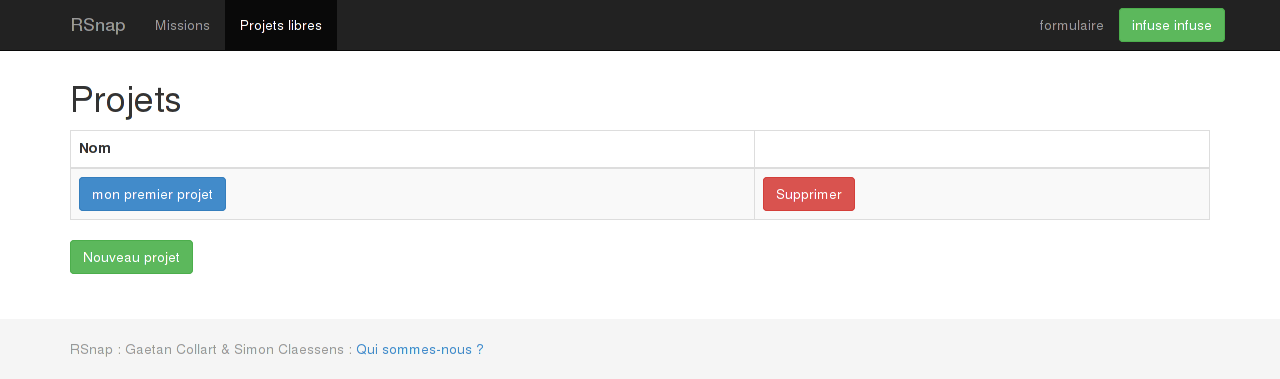
\includegraphics[width=\textwidth]{projet-2}
    \caption{Créeation du programme du projet libre}
    \label{fig:projet-2}
  \end{center}
\end{figure}
